\chapter{Introduction}

Asbestos is a very toxic mineral that comes in one of six types. The most common being chrysotile asbestos, which accounts for over 90\% of all the asbestos commerciall used \cite{asbestosMaacenter}. It has long, curly fibers which can be woven into materials and has many commercial applications. It is very durable, heat and chemical resistant and has strong insulating properties. These are the reasons why asbesots fibers were often used in thousands of products before the toxicity became widely known. There are six main asbestos minerals that are currently regulated but there exist many more mineral forms of asbestos - mainly from the amphibole group \cite{environmental2008framework}. The six different types are chrysotile, amosite, tremolite, crocidolite, anthophyllite and actinolite. Figure \ref{fig:chrysotile} shows chrysotile how it can occur in nature and how it is seen under a scanning electron microscope (SEM).

\begin{figure}[h]
\centering

\subfigure{
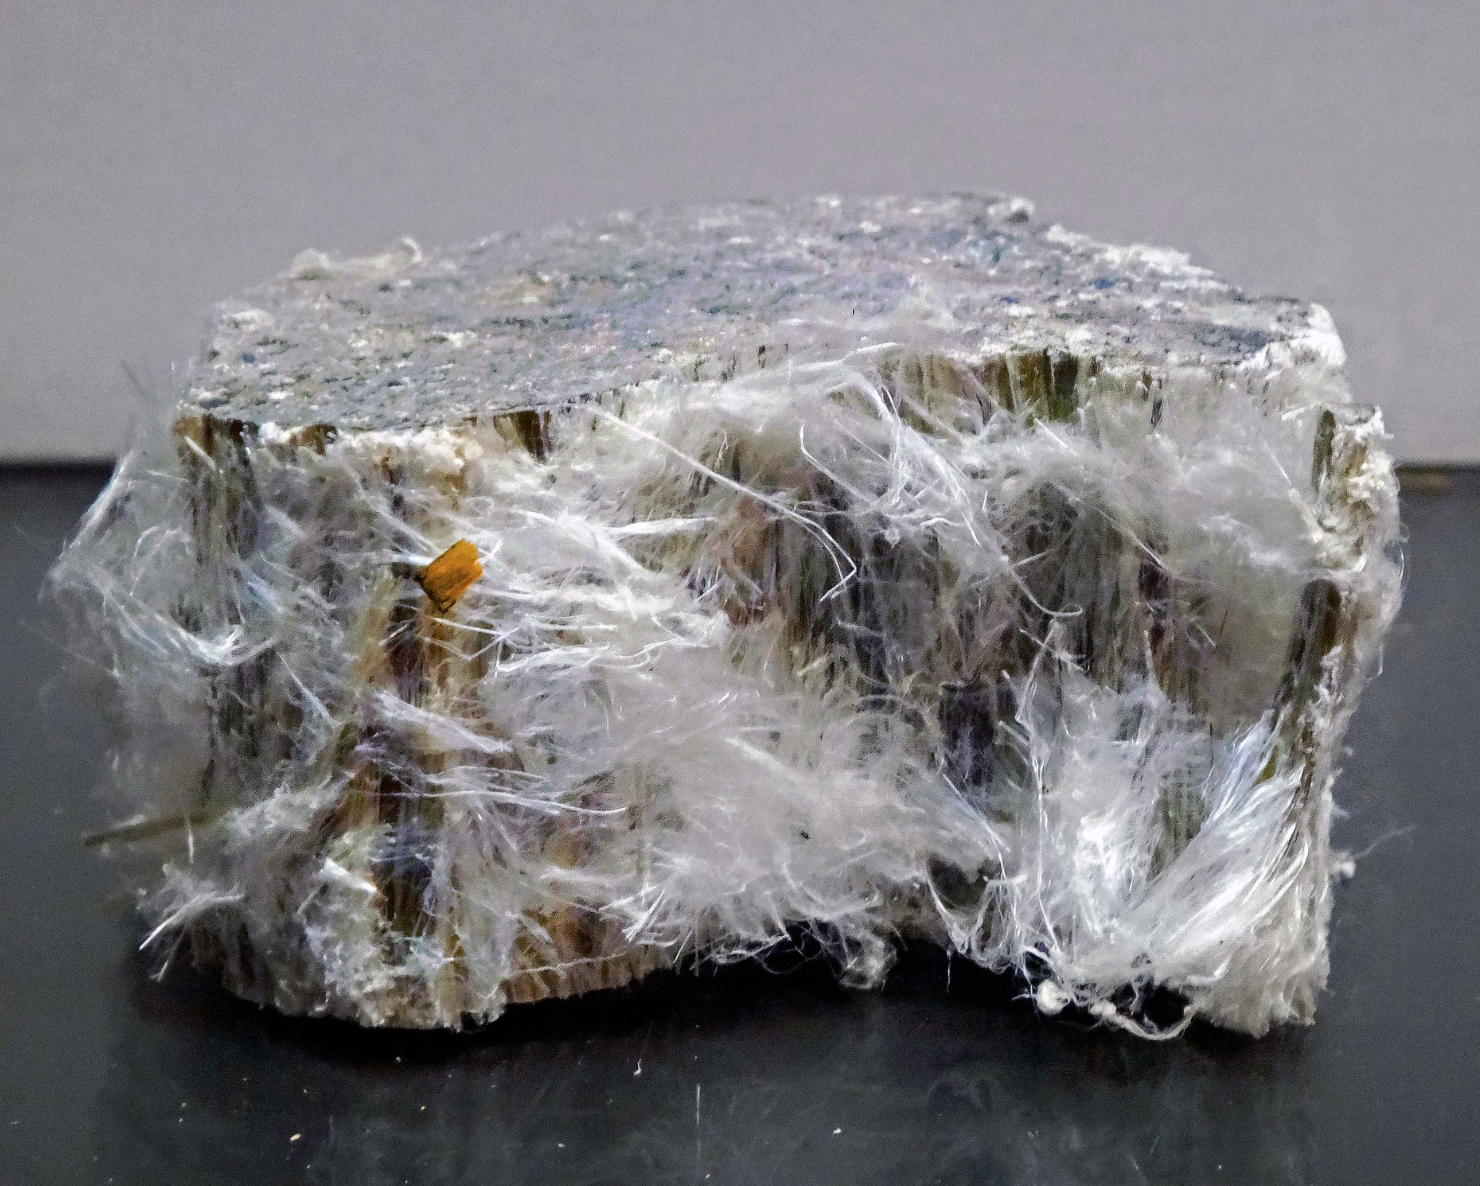
\includegraphics[width=.35\textwidth]{images/chapter1/chrysotileFullSize}
}
\subfigure{
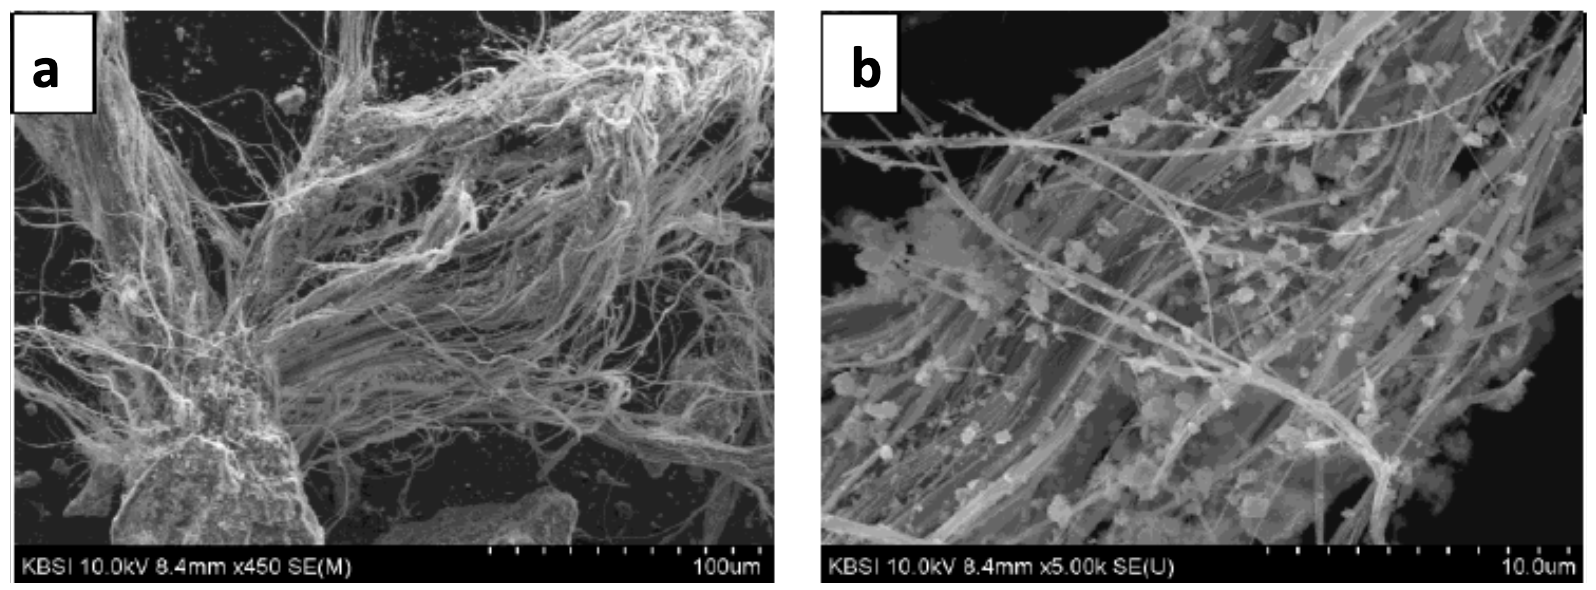
\includegraphics[width=.55\textwidth]{images/chapter1/chrysotileSEM}
}
\caption{On the left side a stone with chrysotile asbesots in a stone is shown \cite{chrysoltileFullSizeImage}. On the right side two images taken by Scanning Electron Microscopy are added for comparison \cite{mohammed2015}. In any case the fiber like structure is very typical for chrysotile asbestos.}
\label{fig:chrysotile}
\end{figure}

Exposure with asbestos through inhalation or ingestion can lead to many asbestos-related diseases like mesothelioma (a type of cancer) or asbestosis (long term inflammation and scarring of the lungs) \cite{asbestosMaacenter, MesotheliomaWiki, asbestosisWiki}. These debilitating health effects in humans after exposure to asbestos made it very necessary to have effective techniques and methods to detect and quantify asbestos in a variety of materials and the environment. There is no one superior method in asbestos detection but rather a large number of different methods that need to be adapted to the specific task at hand. \\

Convolutional Neural Networks (CNNs) have become the standard in many areas such as image recognition, classification, object detection, identifying faces and others. Although CNNs have existed already since 1988, recent progress in computational power through GPU's have made bigger neural networks possible. In 2012, Alex Krizhevsky and his group won the ImageNet Large Scale Visual Recognition Challenge (ILSVRC) with a CNN and since then research into this type of Neural Networks has increased drastically with new CNNs surpassing human performance in many fields. \\

[[ how much references do I need here already?  I think none for the introduction but then again I make many claims that could be challenged when not providing references... ]]

\section{Motivation}

A Convolutional Neural Network is a specific type of an Artifical Neural Network (ANN) which gets its name from trying to model a biological neural network. It consists of many neurons often called nodes or units that process information in a feed forward manner. A neuron receives input from other neurons very similar to brain cells that are interconnected with other brain cells, building up a huge network. The input from many different neurons is weighted and processed before forwarding the information/output to the next neuron. A network is created where many neurons are fully connected to the next layer of neurons leading up to a Multi Layer Perceptron. \\

For image classification having fully connected layers of hidden units is not very useful, since no spatial information can be retrieved from the image itself. Convolutional Neural Networks are able to scan through the image and retrieve spatial feature maps, that find characteristic patterns throughout the image. These convolutional layers are connected to form a bigger and deeper network.  \\

\section{Study Subject}

The goal of this thesis is to find a suitable architecture to recognize asbestos in microscopic images, understand how the architecture works and improve on it, if possible. Also I will do experiments on transfer learning and discuss if it is applicable for this domain of SEM images although the pre-learning has been done on regular real life objects. \\

I will first start with AlexNet to get a good baseline, from which to improve on. Also an Inter-Annotater Agreement Rate will be fixed by letting several subjects classify a certain amount of images. The current state of the art architectures are all based on natural images as found in the ImageNet dataset from the ILSVRC. To achieve good accuracies I will need to understand how the different layers of a CNN interact with each other in order to be able to alter the width, depth and other parameters of an architecture to better suite the given asbestos dataset. The dataloader will need re-implementation since the asbestos images are big images and resizing them leads to losing the fine structure of the asbestos fibers, making it impossible to classify the images correctly. Transfer learning will be applied in order to start with already pre-trained weights. Holding some of the layers fixed and fine-tuning the last couples of layers should improve efficiency and accuracy considerably. In the end I will need to optimize all used hyper-parameters in order to achieve best possible results and run the architecture for a long period of time.

\section{Outline}

The remainder of this thesis is organized as follows. Chapter 2 explains shortly the dataset used for this task, go into related work and make an analysis of what frameworks can be used. Chapter 3 will explain CNN in detail and go  all the architectures used in this thesis and explain them. Chapter 4 will explain how the architecutes are used and altered and what methods are applied. Chapter 5 will evaluate transfer learning, since it is one main contribution of this thesis. Chapter 6 will evaluate changes to the architectures. Chapter 7 will go into the conclusion and further work.
